\documentclass[1p]{elsarticle_modified}
%\bibliographystyle{elsarticle-num}

%\usepackage[colorlinks]{hyperref}
%\usepackage{abbrmath_seonhwa} %\Abb, \Ascr, \Acal ,\Abf, \Afrak
\usepackage{amsfonts}
\usepackage{amssymb}
\usepackage{amsmath}
\usepackage{amsthm}
\usepackage{scalefnt}
\usepackage{amsbsy}
\usepackage{kotex}
\usepackage{caption}
\usepackage{subfig}
\usepackage{color}
\usepackage{graphicx}
\usepackage{xcolor} %% white, black, red, green, blue, cyan, magenta, yellow
\usepackage{float}
\usepackage{setspace}
\usepackage{hyperref}

\usepackage{tikz}
\usetikzlibrary{arrows}

\usepackage{multirow}
\usepackage{array} % fixed length table
\usepackage{hhline}

%%%%%%%%%%%%%%%%%%%%%
\makeatletter
\renewcommand*\env@matrix[1][\arraystretch]{%
	\edef\arraystretch{#1}%
	\hskip -\arraycolsep
	\let\@ifnextchar\new@ifnextchar
	\array{*\c@MaxMatrixCols c}}
\makeatother %https://tex.stackexchange.com/questions/14071/how-can-i-increase-the-line-spacing-in-a-matrix
%%%%%%%%%%%%%%%

\usepackage[normalem]{ulem}

\newcommand{\msout}[1]{\ifmmode\text{\sout{\ensuremath{#1}}}\else\sout{#1}\fi}
%SOURCE: \msout is \stkout macro in https://tex.stackexchange.com/questions/20609/strikeout-in-math-mode

\newcommand{\cancel}[1]{
	\ifmmode
	{\color{red}\msout{#1}}
	\else
	{\color{red}\sout{#1}}
	\fi
}

\newcommand{\add}[1]{
	{\color{blue}\uwave{#1}}
}

\newcommand{\replace}[2]{
	\ifmmode
	{\color{red}\msout{#1}}{\color{blue}\uwave{#2}}
	\else
	{\color{red}\sout{#1}}{\color{blue}\uwave{#2}}
	\fi
}

\newcommand{\Sol}{\mathcal{S}} %segment
\newcommand{\D}{D} %diagram
\newcommand{\A}{\mathcal{A}} %arc


%%%%%%%%%%%%%%%%%%%%%%%%%%%%%5 test

\def\sl{\operatorname{\textup{SL}}(2,\Cbb)}
\def\psl{\operatorname{\textup{PSL}}(2,\Cbb)}
\def\quan{\mkern 1mu \triangleright \mkern 1mu}

\theoremstyle{definition}
\newtheorem{thm}{Theorem}[section]
\newtheorem{prop}[thm]{Proposition}
\newtheorem{lem}[thm]{Lemma}
\newtheorem{ques}[thm]{Question}
\newtheorem{cor}[thm]{Corollary}
\newtheorem{defn}[thm]{Definition}
\newtheorem{exam}[thm]{Example}
\newtheorem{rmk}[thm]{Remark}
\newtheorem{alg}[thm]{Algorithm}

\newcommand{\I}{\sqrt{-1}}
\begin{document}

%\begin{frontmatter}
%
%\title{Boundary parabolic representations of knots up to 8 crossings}
%
%%% Group authors per affiliation:
%\author{Yunhi Cho} 
%\address{Department of Mathematics, University of Seoul, Seoul, Korea}
%\ead{yhcho@uos.ac.kr}
%
%
%\author{Seonhwa Kim} %\fnref{s_kim}}
%\address{Center for Geometry and Physics, Institute for Basic Science, Pohang, 37673, Korea}
%\ead{ryeona17@ibs.re.kr}
%
%\author{Hyuk Kim}
%\address{Department of Mathematical Sciences, Seoul National University, Seoul 08826, Korea}
%\ead{hyukkim@snu.ac.kr}
%
%\author{Seokbeom Yoon}
%\address{Department of Mathematical Sciences, Seoul National University, Seoul, 08826,  Korea}
%\ead{sbyoon15@snu.ac.kr}
%
%\begin{abstract}
%We find all boundary parabolic representation of knots up to 8 crossings.
%
%\end{abstract}
%\begin{keyword}
%    \MSC[2010] 57M25 
%\end{keyword}
%
%\end{frontmatter}

%\linenumbers
%\tableofcontents
%
\newcommand\colored[1]{\textcolor{white}{\rule[-0.35ex]{0.8em}{1.4ex}}\kern-0.8em\color{red} #1}%
%\newcommand\colored[1]{\textcolor{white}{ #1}\kern-2.17ex	\textcolor{white}{ #1}\kern-1.81ex	\textcolor{white}{ #1}\kern-2.15ex\color{red}#1	}

{\Large $\underline{12a_{0351}~(K12a_{0351})}$}

\setlength{\tabcolsep}{10pt}
\renewcommand{\arraystretch}{1.6}
\vspace{1cm}\begin{tabular}{m{100pt}>{\centering\arraybackslash}m{274pt}}
\multirow{5}{120pt}{
	\centering
	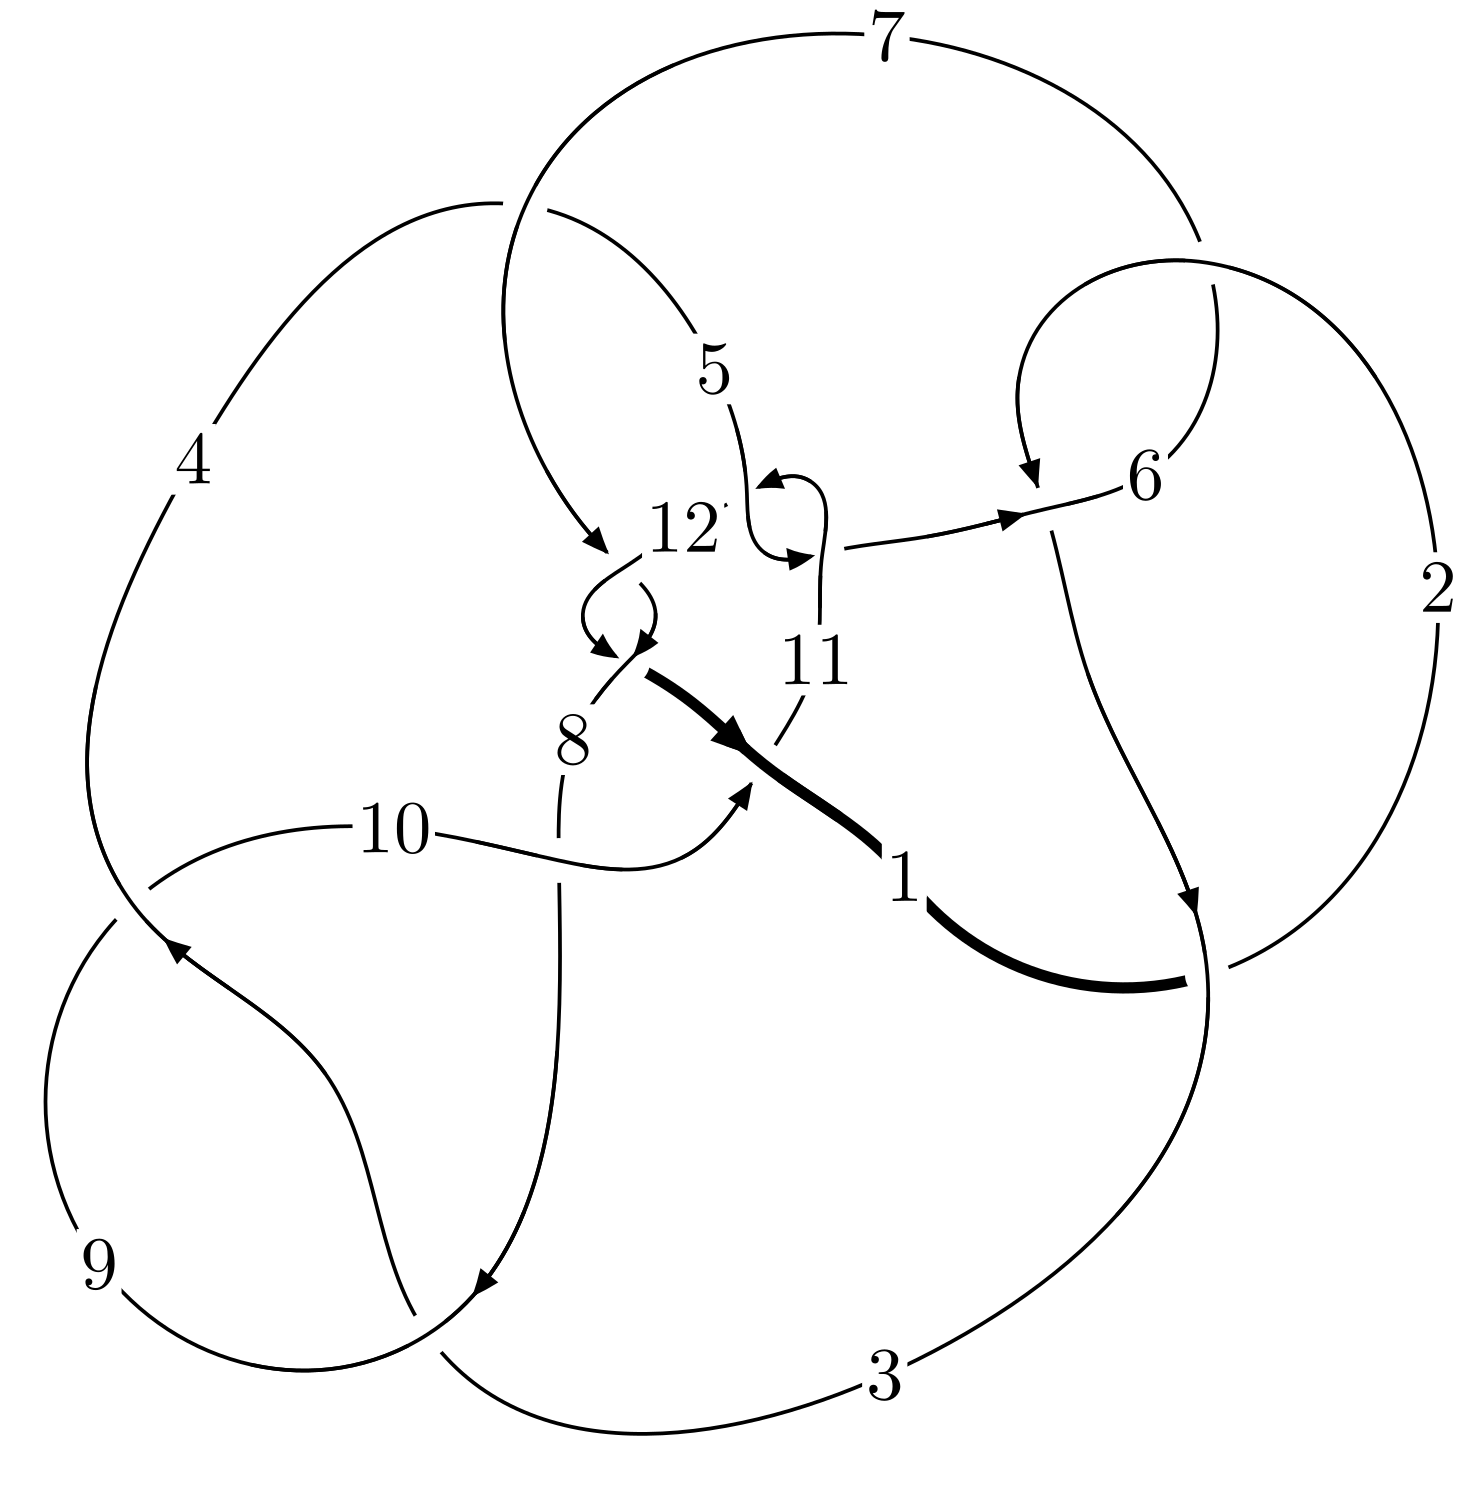
\includegraphics[width=112pt]{../../../GIT/diagram.site/Diagrams/png/1152_12a_0351.png}\\
\ \ \ A knot diagram\footnotemark}&
\allowdisplaybreaks
\textbf{Linearized knot diagam} \\
\cline{2-2}
 &
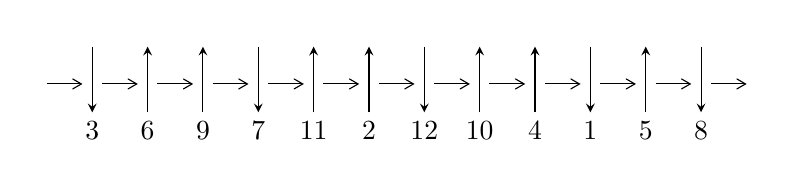
\begin{tikzpicture}[x=20pt, y=17pt]
	% nodes
	\node (C0) at (0, 0) {};
	\node (C1) at (1, 0) {};
	\node (C1U) at (1, +1) {};
	\node (C1D) at (1, -1) {3};

	\node (C2) at (2, 0) {};
	\node (C2U) at (2, +1) {};
	\node (C2D) at (2, -1) {6};

	\node (C3) at (3, 0) {};
	\node (C3U) at (3, +1) {};
	\node (C3D) at (3, -1) {9};

	\node (C4) at (4, 0) {};
	\node (C4U) at (4, +1) {};
	\node (C4D) at (4, -1) {7};

	\node (C5) at (5, 0) {};
	\node (C5U) at (5, +1) {};
	\node (C5D) at (5, -1) {11};

	\node (C6) at (6, 0) {};
	\node (C6U) at (6, +1) {};
	\node (C6D) at (6, -1) {2};

	\node (C7) at (7, 0) {};
	\node (C7U) at (7, +1) {};
	\node (C7D) at (7, -1) {12};

	\node (C8) at (8, 0) {};
	\node (C8U) at (8, +1) {};
	\node (C8D) at (8, -1) {10};

	\node (C9) at (9, 0) {};
	\node (C9U) at (9, +1) {};
	\node (C9D) at (9, -1) {4};

	\node (C10) at (10, 0) {};
	\node (C10U) at (10, +1) {};
	\node (C10D) at (10, -1) {1};

	\node (C11) at (11, 0) {};
	\node (C11U) at (11, +1) {};
	\node (C11D) at (11, -1) {5};

	\node (C12) at (12, 0) {};
	\node (C12U) at (12, +1) {};
	\node (C12D) at (12, -1) {8};
	\node (C13) at (13, 0) {};

	% arrows
	\draw[->,>={angle 60}]
	(C0) edge (C1) (C1) edge (C2) (C2) edge (C3) (C3) edge (C4) (C4) edge (C5) (C5) edge (C6) (C6) edge (C7) (C7) edge (C8) (C8) edge (C9) (C9) edge (C10) (C10) edge (C11) (C11) edge (C12) (C12) edge (C13) ;	\draw[->,>=stealth]
	(C1U) edge (C1D) (C2D) edge (C2U) (C3D) edge (C3U) (C4U) edge (C4D) (C5D) edge (C5U) (C6D) edge (C6U) (C7U) edge (C7D) (C8D) edge (C8U) (C9D) edge (C9U) (C10U) edge (C10D) (C11D) edge (C11U) (C12U) edge (C12D) ;
	\end{tikzpicture} \\
\hhline{~~} \\& 
\textbf{Solving Sequence} \\ \cline{2-2} 
 &
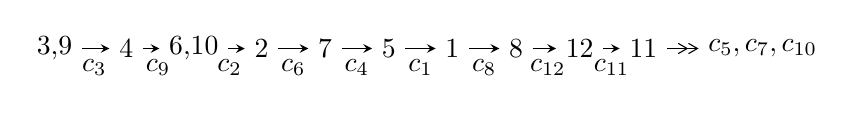
\begin{tikzpicture}[x=23pt, y=7pt]
	% node
	\node (A0) at (-1/8, 0) {3,9};
	\node (A1) at (1, 0) {4};
	\node (A2) at (33/16, 0) {6,10};
	\node (A3) at (25/8, 0) {2};
	\node (A4) at (33/8, 0) {7};
	\node (A5) at (41/8, 0) {5};
	\node (A6) at (49/8, 0) {1};
	\node (A7) at (57/8, 0) {8};
	\node (A8) at (65/8, 0) {12};
	\node (A9) at (73/8, 0) {11};
	\node (C1) at (1/2, -1) {$c_{3}$};
	\node (C2) at (3/2, -1) {$c_{9}$};
	\node (C3) at (21/8, -1) {$c_{2}$};
	\node (C4) at (29/8, -1) {$c_{6}$};
	\node (C5) at (37/8, -1) {$c_{4}$};
	\node (C6) at (45/8, -1) {$c_{1}$};
	\node (C7) at (53/8, -1) {$c_{8}$};
	\node (C8) at (61/8, -1) {$c_{12}$};
	\node (C9) at (69/8, -1) {$c_{11}$};
	\node (A10) at (11, 0) {$c_{5},c_{7},c_{10}$};

	% edge
	\draw[->,>=stealth]	
	(A0) edge (A1) (A1) edge (A2) (A2) edge (A3) (A3) edge (A4) (A4) edge (A5) (A5) edge (A6) (A6) edge (A7) (A7) edge (A8) (A8) edge (A9) ;
	\draw[->>,>={angle 60}]	
	(A9) edge (A10);
\end{tikzpicture} \\ 

\end{tabular} \\

\footnotetext{
The image of knot diagram is generated by the software ``\textbf{Draw programme}" developed by Andrew Bartholomew(\url{http://www.layer8.co.uk/maths/draw/index.htm\#Running-draw}), where we modified some parts for our purpose(\url{https://github.com/CATsTAILs/LinksPainter}).
}\phantom \\ \newline 
\centering \textbf{Ideals for irreducible components\footnotemark of $X_{\text{par}}$} 
 
\begin{align*}
I^u_{1}&=\langle 
8.22708\times10^{260} u^{115}+5.90473\times10^{259} u^{114}+\cdots+7.11945\times10^{261} b+7.95379\times10^{261},\\
\phantom{I^u_{1}}&\phantom{= \langle  }5.48204\times10^{262} u^{115}+3.62166\times10^{262} u^{114}+\cdots+9.25529\times10^{262} a-1.21893\times10^{263},\;u^{116}+u^{115}+\cdots-12 u+4\rangle \\
I^u_{2}&=\langle 
-3 a u+7 b+12 a-5 u+13,\;18 a^2-3 a u+48 a- u+39,\;u^2-2\rangle \\
\\
I^v_{1}&=\langle 
a,\;b- v,\;v^2+v+1\rangle \\
\end{align*}
\raggedright * 3 irreducible components of $\dim_{\mathbb{C}}=0$, with total 122 representations.\\
\footnotetext{All coefficients of polynomials are rational numbers. But the coefficients are sometimes approximated in decimal forms when there is not enough margin.}
\newpage
\renewcommand{\arraystretch}{1}
\centering \section*{I. $I^u_{1}= \langle 8.23\times10^{260} u^{115}+5.90\times10^{259} u^{114}+\cdots+7.12\times10^{261} b+7.95\times10^{261},\;5.48\times10^{262} u^{115}+3.62\times10^{262} u^{114}+\cdots+9.26\times10^{262} a-1.22\times10^{263},\;u^{116}+u^{115}+\cdots-12 u+4 \rangle$}
\flushleft \textbf{(i) Arc colorings}\\
\begin{tabular}{m{7pt} m{180pt} m{7pt} m{180pt} }
\flushright $a_{3}=$&$\begin{pmatrix}1\\0\end{pmatrix}$ \\
\flushright $a_{9}=$&$\begin{pmatrix}0\\u\end{pmatrix}$ \\
\flushright $a_{4}=$&$\begin{pmatrix}1\\- u^2\end{pmatrix}$ \\
\flushright $a_{6}=$&$\begin{pmatrix}-0.592314 u^{115}-0.391307 u^{114}+\cdots+4.00136 u+1.31701\\-0.115558 u^{115}-0.00829380 u^{114}+\cdots+6.41816 u-1.11719\end{pmatrix}$ \\
\flushright $a_{10}=$&$\begin{pmatrix}u\\- u^3+u\end{pmatrix}$ \\
\flushright $a_{2}=$&$\begin{pmatrix}-0.0576376 u^{115}-0.341529 u^{114}+\cdots+2.70043 u+6.41023\\-0.109926 u^{115}-0.000292556 u^{114}+\cdots+5.86706 u-2.13299\end{pmatrix}$ \\
\flushright $a_{7}=$&$\begin{pmatrix}-0.624496 u^{115}-0.335359 u^{114}+\cdots+13.6484 u+4.37568\\0.130256 u^{115}+0.108791 u^{114}+\cdots+2.77584 u-1.42974\end{pmatrix}$ \\
\flushright $a_{5}=$&$\begin{pmatrix}0.918893 u^{115}+0.826941 u^{114}+\cdots+5.11609 u-0.840015\\0.278228 u^{115}+0.0809501 u^{114}+\cdots-9.46479 u+0.173513\end{pmatrix}$ \\
\flushright $a_{1}=$&$\begin{pmatrix}-0.167564 u^{115}-0.341822 u^{114}+\cdots+8.56749 u+4.27725\\-0.109926 u^{115}-0.000292556 u^{114}+\cdots+5.86706 u-2.13299\end{pmatrix}$ \\
\flushright $a_{8}=$&$\begin{pmatrix}- u^3\\u^5- u^3+u\end{pmatrix}$ \\
\flushright $a_{12}=$&$\begin{pmatrix}-0.105593 u^{115}-0.334986 u^{114}+\cdots+6.85446 u+4.76672\\-0.132149 u^{115}+0.0239453 u^{114}+\cdots+5.21273 u-2.20714\end{pmatrix}$ \\
\flushright $a_{11}=$&$\begin{pmatrix}0.453168 u^{115}+0.309762 u^{114}+\cdots-5.33012 u-6.99372\\-0.199402 u^{115}-0.129061 u^{114}+\cdots+1.83081 u+0.396491\end{pmatrix}$\\&\end{tabular}
\flushleft \textbf{(ii) Obstruction class $= -1$}\\~\\
\flushleft \textbf{(iii) Cusp Shapes $= 1.30353 u^{115}+0.380419 u^{114}+\cdots-48.9228 u+9.39672$}\\~\\
\newpage\renewcommand{\arraystretch}{1}
\flushleft \textbf{(iv) u-Polynomials at the component}\newline \\
\begin{tabular}{m{50pt}|m{274pt}}
Crossings & \hspace{64pt}u-Polynomials at each crossing \\
\hline $$\begin{aligned}c_{1}\end{aligned}$$&$\begin{aligned}
&u^{116}+52 u^{115}+\cdots-5438 u+289
\end{aligned}$\\
\hline $$\begin{aligned}c_{2},c_{6}\end{aligned}$$&$\begin{aligned}
&u^{116}-2 u^{115}+\cdots+44 u+17
\end{aligned}$\\
\hline $$\begin{aligned}c_{3},c_{9}\end{aligned}$$&$\begin{aligned}
&u^{116}+u^{115}+\cdots-12 u+4
\end{aligned}$\\
\hline $$\begin{aligned}c_{4}\end{aligned}$$&$\begin{aligned}
&28561(28561 u^{116}-153790 u^{115}+\cdots-8.25675\times10^{8} u+3.49024\times10^{7})
\end{aligned}$\\
\hline $$\begin{aligned}c_{5},c_{11}\end{aligned}$$&$\begin{aligned}
&u^{116}+u^{115}+\cdots+44 u+4
\end{aligned}$\\
\hline $$\begin{aligned}c_{7},c_{12}\end{aligned}$$&$\begin{aligned}
&u^{116}+3 u^{115}+\cdots-989 u+343
\end{aligned}$\\
\hline $$\begin{aligned}c_{8}\end{aligned}$$&$\begin{aligned}
&u^{116}-51 u^{115}+\cdots-304 u+16
\end{aligned}$\\
\hline $$\begin{aligned}c_{10}\end{aligned}$$&$\begin{aligned}
&28561(28561 u^{116}+173563 u^{115}+\cdots-6624257 u+463351)
\end{aligned}$\\
\hline
\end{tabular}\\~\\
\newpage\renewcommand{\arraystretch}{1}
\flushleft \textbf{(v) Riley Polynomials at the component}\newline \\
\begin{tabular}{m{50pt}|m{274pt}}
Crossings & \hspace{64pt}Riley Polynomials at each crossing \\
\hline $$\begin{aligned}c_{1}\end{aligned}$$&$\begin{aligned}
&y^{116}+28 y^{115}+\cdots-20164894 y+83521
\end{aligned}$\\
\hline $$\begin{aligned}c_{2},c_{6}\end{aligned}$$&$\begin{aligned}
&y^{116}+52 y^{115}+\cdots-5438 y+289
\end{aligned}$\\
\hline $$\begin{aligned}c_{3},c_{9}\end{aligned}$$&$\begin{aligned}
&y^{116}-51 y^{115}+\cdots-304 y+16
\end{aligned}$\\
\hline $$\begin{aligned}c_{4}\end{aligned}$$&$\begin{aligned}
&815730721\\
&\cdot(8.16\times10^{8} y^{116}-2.56\times10^{10} y^{115}+\cdots+3.19\times10^{16} y+1.22\times10^{15})
\end{aligned}$\\
\hline $$\begin{aligned}c_{5},c_{11}\end{aligned}$$&$\begin{aligned}
&y^{116}+69 y^{115}+\cdots+80 y+16
\end{aligned}$\\
\hline $$\begin{aligned}c_{7},c_{12}\end{aligned}$$&$\begin{aligned}
&y^{116}-93 y^{115}+\cdots-1659319 y+117649
\end{aligned}$\\
\hline $$\begin{aligned}c_{8}\end{aligned}$$&$\begin{aligned}
&y^{116}+33 y^{115}+\cdots-4864 y+256
\end{aligned}$\\
\hline $$\begin{aligned}c_{10}\end{aligned}$$&$\begin{aligned}
&815730721\\
&\cdot(8.16\times10^{8} y^{116}-5.43\times10^{10} y^{115}+\cdots-1.02\times10^{13} y+2.15\times10^{11})
\end{aligned}$\\
\hline
\end{tabular}\\~\\
\newpage\flushleft \textbf{(vi) Complex Volumes and Cusp Shapes}
$$\begin{array}{c|c|c}  
\text{Solutions to }I^u_{1}& \I (\text{vol} + \sqrt{-1}CS) & \text{Cusp shape}\\
 \hline 
\begin{aligned}
u &= -0.466716 + 0.884426 I \\
a &= -0.783595 - 0.126337 I \\
b &= \phantom{-}0.653585 - 0.363267 I\end{aligned}
 & -2.67219 + 1.89988 I & \phantom{-0.000000 } 0 \\ \hline\begin{aligned}
u &= -0.466716 - 0.884426 I \\
a &= -0.783595 + 0.126337 I \\
b &= \phantom{-}0.653585 + 0.363267 I\end{aligned}
 & -2.67219 - 1.89988 I & \phantom{-0.000000 } 0 \\ \hline\begin{aligned}
u &= \phantom{-}0.833896 + 0.554451 I \\
a &= -0.727306 - 0.756093 I \\
b &= \phantom{-}0.541090 - 1.019580 I\end{aligned}
 & -2.32060 + 0.05845 I & \phantom{-0.000000 } 0 \\ \hline\begin{aligned}
u &= \phantom{-}0.833896 - 0.554451 I \\
a &= -0.727306 + 0.756093 I \\
b &= \phantom{-}0.541090 + 1.019580 I\end{aligned}
 & -2.32060 - 0.05845 I & \phantom{-0.000000 } 0 \\ \hline\begin{aligned}
u &= \phantom{-}0.515699 + 0.858960 I \\
a &= \phantom{-}0.768671 + 0.054540 I \\
b &= -0.664056 + 0.147665 I\end{aligned}
 & -6.86951 + 3.26307 I & \phantom{-0.000000 } 0 \\ \hline\begin{aligned}
u &= \phantom{-}0.515699 - 0.858960 I \\
a &= \phantom{-}0.768671 - 0.054540 I \\
b &= -0.664056 - 0.147665 I\end{aligned}
 & -6.86951 - 3.26307 I & \phantom{-0.000000 } 0 \\ \hline\begin{aligned}
u &= -0.796622 + 0.599234 I \\
a &= -0.234219 + 0.406414 I \\
b &= -0.68922 - 1.38197 I\end{aligned}
 & -5.98756 + 0.45829 I & \phantom{-0.000000 } 0 \\ \hline\begin{aligned}
u &= -0.796622 - 0.599234 I \\
a &= -0.234219 - 0.406414 I \\
b &= -0.68922 + 1.38197 I\end{aligned}
 & -5.98756 - 0.45829 I & \phantom{-0.000000 } 0 \\ \hline\begin{aligned}
u &= \phantom{-}0.496277 + 0.882378 I \\
a &= \phantom{-}0.683895 - 0.105274 I \\
b &= -0.921430 - 0.377905 I\end{aligned}
 & -6.72237 - 7.44661 I & \phantom{-0.000000 } 0 \\ \hline\begin{aligned}
u &= \phantom{-}0.496277 - 0.882378 I \\
a &= \phantom{-}0.683895 + 0.105274 I \\
b &= -0.921430 + 0.377905 I\end{aligned}
 & -6.72237 + 7.44661 I & \phantom{-0.000000 } 0\\
 \hline 
 \end{array}$$\newpage$$\begin{array}{c|c|c}  
\text{Solutions to }I^u_{1}& \I (\text{vol} + \sqrt{-1}CS) & \text{Cusp shape}\\
 \hline 
\begin{aligned}
u &= -0.821230 + 0.618768 I \\
a &= -0.794720 - 1.140120 I \\
b &= \phantom{-}0.261743 - 0.895424 I\end{aligned}
 & -2.04215 - 2.50988 I & \phantom{-0.000000 } 0 \\ \hline\begin{aligned}
u &= -0.821230 - 0.618768 I \\
a &= -0.794720 + 1.140120 I \\
b &= \phantom{-}0.261743 + 0.895424 I\end{aligned}
 & -2.04215 + 2.50988 I & \phantom{-0.000000 } 0 \\ \hline\begin{aligned}
u &= \phantom{-}0.872725 + 0.555380 I \\
a &= \phantom{-}2.93230 - 0.92577 I \\
b &= -0.622964 - 0.983728 I\end{aligned}
 & -2.19443 + 4.38805 I & \phantom{-0.000000 } 0 \\ \hline\begin{aligned}
u &= \phantom{-}0.872725 - 0.555380 I \\
a &= \phantom{-}2.93230 + 0.92577 I \\
b &= -0.622964 + 0.983728 I\end{aligned}
 & -2.19443 - 4.38805 I & \phantom{-0.000000 } 0 \\ \hline\begin{aligned}
u &= -0.314014 + 0.987232 I \\
a &= \phantom{-}0.779419 - 0.361334 I \\
b &= -0.337968 - 1.111900 I\end{aligned}
 & -10.48240 + 0.02403 I & \phantom{-0.000000 } 0 \\ \hline\begin{aligned}
u &= -0.314014 - 0.987232 I \\
a &= \phantom{-}0.779419 + 0.361334 I \\
b &= -0.337968 + 1.111900 I\end{aligned}
 & -10.48240 - 0.02403 I & \phantom{-0.000000 } 0 \\ \hline\begin{aligned}
u &= -0.835930 + 0.617038 I \\
a &= -0.597118 - 0.860842 I \\
b &= -0.061420 - 0.822216 I\end{aligned}
 & -2.00858 - 2.35815 I & \phantom{-0.000000 } 0 \\ \hline\begin{aligned}
u &= -0.835930 - 0.617038 I \\
a &= -0.597118 + 0.860842 I \\
b &= -0.061420 + 0.822216 I\end{aligned}
 & -2.00858 + 2.35815 I & \phantom{-0.000000 } 0 \\ \hline\begin{aligned}
u &= \phantom{-}0.838690 + 0.617546 I \\
a &= \phantom{-}1.269560 - 0.256708 I \\
b &= -0.09071 - 1.52895 I\end{aligned}
 & -6.41289 + 2.42988 I & \phantom{-0.000000 } 0 \\ \hline\begin{aligned}
u &= \phantom{-}0.838690 - 0.617546 I \\
a &= \phantom{-}1.269560 + 0.256708 I \\
b &= -0.09071 + 1.52895 I\end{aligned}
 & -6.41289 - 2.42988 I & \phantom{-0.000000 } 0\\
 \hline 
 \end{array}$$\newpage$$\begin{array}{c|c|c}  
\text{Solutions to }I^u_{1}& \I (\text{vol} + \sqrt{-1}CS) & \text{Cusp shape}\\
 \hline 
\begin{aligned}
u &= \phantom{-}1.041140 + 0.185992 I \\
a &= -1.83112 - 0.13921 I \\
b &= \phantom{-}0.815154 + 0.555869 I\end{aligned}
 & \phantom{-}3.19024 - 0.63993 I & \phantom{-0.000000 } 0 \\ \hline\begin{aligned}
u &= \phantom{-}1.041140 - 0.185992 I \\
a &= -1.83112 + 0.13921 I \\
b &= \phantom{-}0.815154 - 0.555869 I\end{aligned}
 & \phantom{-}3.19024 + 0.63993 I & \phantom{-0.000000 } 0 \\ \hline\begin{aligned}
u &= -0.640644 + 0.848844 I \\
a &= \phantom{-}0.735683 + 0.692782 I \\
b &= -0.112380 + 1.305980 I\end{aligned}
 & -12.68570 + 4.21380 I & \phantom{-0.000000 } 0 \\ \hline\begin{aligned}
u &= -0.640644 - 0.848844 I \\
a &= \phantom{-}0.735683 - 0.692782 I \\
b &= -0.112380 - 1.305980 I\end{aligned}
 & -12.68570 - 4.21380 I & \phantom{-0.000000 } 0 \\ \hline\begin{aligned}
u &= -0.883251 + 0.602570 I \\
a &= -2.08121 - 0.54168 I \\
b &= \phantom{-}0.83111 - 1.31723 I\end{aligned}
 & -5.71767 - 5.21650 I & \phantom{-0.000000 } 0 \\ \hline\begin{aligned}
u &= -0.883251 - 0.602570 I \\
a &= -2.08121 + 0.54168 I \\
b &= \phantom{-}0.83111 + 1.31723 I\end{aligned}
 & -5.71767 + 5.21650 I & \phantom{-0.000000 } 0 \\ \hline\begin{aligned}
u &= -0.995874 + 0.401809 I \\
a &= -0.71960 - 2.00101 I \\
b &= \phantom{-}0.329550 + 0.745071 I\end{aligned}
 & -1.73973 - 1.33290 I & \phantom{-0.000000 } 0 \\ \hline\begin{aligned}
u &= -0.995874 - 0.401809 I \\
a &= -0.71960 + 2.00101 I \\
b &= \phantom{-}0.329550 - 0.745071 I\end{aligned}
 & -1.73973 + 1.33290 I & \phantom{-0.000000 } 0 \\ \hline\begin{aligned}
u &= -0.495701 + 0.956635 I \\
a &= \phantom{-}0.742573 - 0.406437 I \\
b &= -0.634931 - 1.162860 I\end{aligned}
 & -9.1087 + 13.1311 I & \phantom{-0.000000 } 0 \\ \hline\begin{aligned}
u &= -0.495701 - 0.956635 I \\
a &= \phantom{-}0.742573 + 0.406437 I \\
b &= -0.634931 + 1.162860 I\end{aligned}
 & -9.1087 - 13.1311 I & \phantom{-0.000000 } 0\\
 \hline 
 \end{array}$$\newpage$$\begin{array}{c|c|c}  
\text{Solutions to }I^u_{1}& \I (\text{vol} + \sqrt{-1}CS) & \text{Cusp shape}\\
 \hline 
\begin{aligned}
u &= -0.775905 + 0.497045 I \\
a &= -0.165278 - 0.775090 I \\
b &= -0.238451 - 0.070476 I\end{aligned}
 & -1.78328 - 2.08266 I & \phantom{-0.000000 } 0 \\ \hline\begin{aligned}
u &= -0.775905 - 0.497045 I \\
a &= -0.165278 + 0.775090 I \\
b &= -0.238451 + 0.070476 I\end{aligned}
 & -1.78328 + 2.08266 I & \phantom{-0.000000 } 0 \\ \hline\begin{aligned}
u &= \phantom{-}0.494221 + 0.759596 I \\
a &= \phantom{-}0.307685 + 0.600397 I \\
b &= -0.590578 + 1.186130 I\end{aligned}
 & -3.60510 - 7.79415 I & \phantom{-0.000000 } 0 \\ \hline\begin{aligned}
u &= \phantom{-}0.494221 - 0.759596 I \\
a &= \phantom{-}0.307685 - 0.600397 I \\
b &= -0.590578 - 1.186130 I\end{aligned}
 & -3.60510 + 7.79415 I & \phantom{-0.000000 } 0 \\ \hline\begin{aligned}
u &= -0.779427 + 0.450974 I \\
a &= \phantom{-}0.39113 + 1.97543 I \\
b &= -0.670300 - 0.709245 I\end{aligned}
 & -1.32894 + 0.70219 I & \phantom{-0.000000 } 0 \\ \hline\begin{aligned}
u &= -0.779427 - 0.450974 I \\
a &= \phantom{-}0.39113 - 1.97543 I \\
b &= -0.670300 + 0.709245 I\end{aligned}
 & -1.32894 - 0.70219 I & \phantom{-0.000000 } 0 \\ \hline\begin{aligned}
u &= -0.957835 + 0.541099 I \\
a &= -0.955456 + 0.073183 I \\
b &= \phantom{-}0.723527 - 0.452906 I\end{aligned}
 & -0.57651 - 4.79475 I & \phantom{-0.000000 } 0 \\ \hline\begin{aligned}
u &= -0.957835 - 0.541099 I \\
a &= -0.955456 - 0.073183 I \\
b &= \phantom{-}0.723527 + 0.452906 I\end{aligned}
 & -0.57651 + 4.79475 I & \phantom{-0.000000 } 0 \\ \hline\begin{aligned}
u &= \phantom{-}0.713321 + 0.547036 I \\
a &= -0.287533 + 1.169400 I \\
b &= \phantom{-}1.054150 - 0.828225 I\end{aligned}
 & -4.19877 - 2.44712 I & \phantom{-0.000000 } 0 \\ \hline\begin{aligned}
u &= \phantom{-}0.713321 - 0.547036 I \\
a &= -0.287533 - 1.169400 I \\
b &= \phantom{-}1.054150 + 0.828225 I\end{aligned}
 & -4.19877 + 2.44712 I & \phantom{-0.000000 } 0\\
 \hline 
 \end{array}$$\newpage$$\begin{array}{c|c|c}  
\text{Solutions to }I^u_{1}& \I (\text{vol} + \sqrt{-1}CS) & \text{Cusp shape}\\
 \hline 
\begin{aligned}
u &= \phantom{-}0.943567 + 0.584400 I \\
a &= \phantom{-}1.68583 - 0.51157 I \\
b &= -1.159030 - 0.663749 I\end{aligned}
 & -3.47234 + 7.03624 I & \phantom{-0.000000 } 0 \\ \hline\begin{aligned}
u &= \phantom{-}0.943567 - 0.584400 I \\
a &= \phantom{-}1.68583 + 0.51157 I \\
b &= -1.159030 + 0.663749 I\end{aligned}
 & -3.47234 - 7.03624 I & \phantom{-0.000000 } 0 \\ \hline\begin{aligned}
u &= \phantom{-}0.942127 + 0.604306 I \\
a &= \phantom{-}1.162640 - 0.293149 I \\
b &= \phantom{-}0.439750 - 0.953612 I\end{aligned}
 & -2.77882 - 0.58975 I & \phantom{-0.000000 } 0 \\ \hline\begin{aligned}
u &= \phantom{-}0.942127 - 0.604306 I \\
a &= \phantom{-}1.162640 + 0.293149 I \\
b &= \phantom{-}0.439750 + 0.953612 I\end{aligned}
 & -2.77882 + 0.58975 I & \phantom{-0.000000 } 0 \\ \hline\begin{aligned}
u &= -1.117360 + 0.069621 I \\
a &= -1.28817 - 1.08342 I \\
b &= \phantom{-}0.642708 + 1.046490 I\end{aligned}
 & \phantom{-}1.70184 + 6.08053 I & \phantom{-0.000000 } 0 \\ \hline\begin{aligned}
u &= -1.117360 - 0.069621 I \\
a &= -1.28817 + 1.08342 I \\
b &= \phantom{-}0.642708 - 1.046490 I\end{aligned}
 & \phantom{-}1.70184 - 6.08053 I & \phantom{-0.000000 } 0 \\ \hline\begin{aligned}
u &= \phantom{-}0.832789 + 0.225789 I \\
a &= -0.601053 + 0.233524 I \\
b &= \phantom{-}0.550015 + 0.084883 I\end{aligned}
 & \phantom{-}1.292750 + 0.325346 I & \phantom{-0.000000 } 0 \\ \hline\begin{aligned}
u &= \phantom{-}0.832789 - 0.225789 I \\
a &= -0.601053 - 0.233524 I \\
b &= \phantom{-}0.550015 - 0.084883 I\end{aligned}
 & \phantom{-}1.292750 - 0.325346 I & \phantom{-0.000000 } 0 \\ \hline\begin{aligned}
u &= \phantom{-}0.670876 + 0.535881 I \\
a &= \phantom{-}0.90736 + 2.57743 I \\
b &= -0.366397 + 0.954160 I\end{aligned}
 & -3.79397 - 0.49844 I & \phantom{-0.000000 } 0 \\ \hline\begin{aligned}
u &= \phantom{-}0.670876 - 0.535881 I \\
a &= \phantom{-}0.90736 - 2.57743 I \\
b &= -0.366397 - 0.954160 I\end{aligned}
 & -3.79397 + 0.49844 I & \phantom{-0.000000 } 0\\
 \hline 
 \end{array}$$\newpage$$\begin{array}{c|c|c}  
\text{Solutions to }I^u_{1}& \I (\text{vol} + \sqrt{-1}CS) & \text{Cusp shape}\\
 \hline 
\begin{aligned}
u &= \phantom{-}0.484795 + 1.034740 I \\
a &= -0.722748 - 0.354639 I \\
b &= \phantom{-}0.551009 - 1.081070 I\end{aligned}
 & -4.70990 - 6.59407 I & \phantom{-0.000000 } 0 \\ \hline\begin{aligned}
u &= \phantom{-}0.484795 - 1.034740 I \\
a &= -0.722748 + 0.354639 I \\
b &= \phantom{-}0.551009 + 1.081070 I\end{aligned}
 & -4.70990 + 6.59407 I & \phantom{-0.000000 } 0 \\ \hline\begin{aligned}
u &= \phantom{-}0.555186 + 0.644462 I \\
a &= \phantom{-}0.004936 - 0.922208 I \\
b &= -0.449425 - 1.037710 I\end{aligned}
 & -3.82491 + 5.40390 I & \phantom{-0.000000 } 0 \\ \hline\begin{aligned}
u &= \phantom{-}0.555186 - 0.644462 I \\
a &= \phantom{-}0.004936 + 0.922208 I \\
b &= -0.449425 + 1.037710 I\end{aligned}
 & -3.82491 - 5.40390 I & \phantom{-0.000000 } 0 \\ \hline\begin{aligned}
u &= \phantom{-}1.016380 + 0.540681 I \\
a &= -3.12129 + 0.64540 I \\
b &= \phantom{-}0.461647 + 0.967079 I\end{aligned}
 & -2.64987 + 4.84972 I & \phantom{-0.000000 } 0 \\ \hline\begin{aligned}
u &= \phantom{-}1.016380 - 0.540681 I \\
a &= -3.12129 - 0.64540 I \\
b &= \phantom{-}0.461647 - 0.967079 I\end{aligned}
 & -2.64987 - 4.84972 I & \phantom{-0.000000 } 0 \\ \hline\begin{aligned}
u &= -1.024480 + 0.567357 I \\
a &= -0.768018 - 1.100840 I \\
b &= \phantom{-}1.056100 + 0.312277 I\end{aligned}
 & \phantom{-}0.82781 - 7.00319 I & \phantom{-0.000000 } 0 \\ \hline\begin{aligned}
u &= -1.024480 - 0.567357 I \\
a &= -0.768018 + 1.100840 I \\
b &= \phantom{-}1.056100 - 0.312277 I\end{aligned}
 & \phantom{-}0.82781 + 7.00319 I & \phantom{-0.000000 } 0 \\ \hline\begin{aligned}
u &= -0.592343 + 1.011110 I \\
a &= \phantom{-}0.918671 + 0.496773 I \\
b &= -0.481119 + 1.110180 I\end{aligned}
 & -9.55063 - 7.53106 I & \phantom{-0.000000 } 0 \\ \hline\begin{aligned}
u &= -0.592343 - 1.011110 I \\
a &= \phantom{-}0.918671 - 0.496773 I \\
b &= -0.481119 - 1.110180 I\end{aligned}
 & -9.55063 + 7.53106 I & \phantom{-0.000000 } 0\\
 \hline 
 \end{array}$$\newpage$$\begin{array}{c|c|c}  
\text{Solutions to }I^u_{1}& \I (\text{vol} + \sqrt{-1}CS) & \text{Cusp shape}\\
 \hline 
\begin{aligned}
u &= \phantom{-}1.054510 + 0.527628 I \\
a &= \phantom{-}0.612085 - 1.147380 I \\
b &= -0.787200 + 0.516832 I\end{aligned}
 & \phantom{-}3.25793 + 3.13597 I & \phantom{-0.000000 } 0 \\ \hline\begin{aligned}
u &= \phantom{-}1.054510 - 0.527628 I \\
a &= \phantom{-}0.612085 + 1.147380 I \\
b &= -0.787200 - 0.516832 I\end{aligned}
 & \phantom{-}3.25793 - 3.13597 I & \phantom{-0.000000 } 0 \\ \hline\begin{aligned}
u &= -1.151090 + 0.257276 I \\
a &= \phantom{-}1.87268 - 0.39708 I \\
b &= -0.691766 + 0.756944 I\end{aligned}
 & \phantom{-}4.99239 - 4.08939 I & \phantom{-0.000000 } 0 \\ \hline\begin{aligned}
u &= -1.151090 - 0.257276 I \\
a &= \phantom{-}1.87268 + 0.39708 I \\
b &= -0.691766 - 0.756944 I\end{aligned}
 & \phantom{-}4.99239 + 4.08939 I & \phantom{-0.000000 } 0 \\ \hline\begin{aligned}
u &= \phantom{-}0.736999 + 0.921312 I \\
a &= -1.021070 + 0.667460 I \\
b &= \phantom{-}0.245911 + 1.047670 I\end{aligned}
 & -6.68894 + 0.36281 I & \phantom{-0.000000 } 0 \\ \hline\begin{aligned}
u &= \phantom{-}0.736999 - 0.921312 I \\
a &= -1.021070 - 0.667460 I \\
b &= \phantom{-}0.245911 - 1.047670 I\end{aligned}
 & -6.68894 - 0.36281 I & \phantom{-0.000000 } 0 \\ \hline\begin{aligned}
u &= -0.416152 + 0.702982 I \\
a &= -0.657214 + 0.652284 I \\
b &= \phantom{-}0.550081 + 1.020460 I\end{aligned}
 & -0.25960 + 3.42242 I & \phantom{-0.000000 } 0 \\ \hline\begin{aligned}
u &= -0.416152 - 0.702982 I \\
a &= -0.657214 - 0.652284 I \\
b &= \phantom{-}0.550081 - 1.020460 I\end{aligned}
 & -0.25960 - 3.42242 I & \phantom{-0.000000 } 0 \\ \hline\begin{aligned}
u &= \phantom{-}1.190070 + 0.157741 I \\
a &= \phantom{-}1.33756 - 0.93877 I \\
b &= -0.634540 + 0.887405 I\end{aligned}
 & \phantom{-}4.59187 - 1.01993 I & \phantom{-0.000000 } 0 \\ \hline\begin{aligned}
u &= \phantom{-}1.190070 - 0.157741 I \\
a &= \phantom{-}1.33756 + 0.93877 I \\
b &= -0.634540 - 0.887405 I\end{aligned}
 & \phantom{-}4.59187 + 1.01993 I & \phantom{-0.000000 } 0\\
 \hline 
 \end{array}$$\newpage$$\begin{array}{c|c|c}  
\text{Solutions to }I^u_{1}& \I (\text{vol} + \sqrt{-1}CS) & \text{Cusp shape}\\
 \hline 
\begin{aligned}
u &= -1.075010 + 0.604590 I \\
a &= \phantom{-}2.23506 + 0.54337 I \\
b &= -0.625953 + 1.067030 I\end{aligned}
 & \phantom{-}1.59755 - 8.45756 I & \phantom{-0.000000 } 0 \\ \hline\begin{aligned}
u &= -1.075010 - 0.604590 I \\
a &= \phantom{-}2.23506 - 0.54337 I \\
b &= -0.625953 - 1.067030 I\end{aligned}
 & \phantom{-}1.59755 + 8.45756 I & \phantom{-0.000000 } 0 \\ \hline\begin{aligned}
u &= -0.755200 + 0.125730 I \\
a &= \phantom{-}0.54008 + 1.48819 I \\
b &= -0.787063 - 0.237062 I\end{aligned}
 & -1.07137 + 2.52393 I & \phantom{-}3.16937 - 4.49551 I \\ \hline\begin{aligned}
u &= -0.755200 - 0.125730 I \\
a &= \phantom{-}0.54008 - 1.48819 I \\
b &= -0.787063 + 0.237062 I\end{aligned}
 & -1.07137 - 2.52393 I & \phantom{-}3.16937 + 4.49551 I \\ \hline\begin{aligned}
u &= \phantom{-}1.203200 + 0.280770 I \\
a &= -0.617584 + 0.816387 I \\
b &= \phantom{-}0.118500 - 0.988627 I\end{aligned}
 & -5.27584 + 3.81255 I & \phantom{-0.000000 } 0 \\ \hline\begin{aligned}
u &= \phantom{-}1.203200 - 0.280770 I \\
a &= -0.617584 - 0.816387 I \\
b &= \phantom{-}0.118500 + 0.988627 I\end{aligned}
 & -5.27584 - 3.81255 I & \phantom{-0.000000 } 0 \\ \hline\begin{aligned}
u &= -1.239360 + 0.011306 I \\
a &= -1.72127 + 0.47650 I \\
b &= \phantom{-}0.754990 - 0.485834 I\end{aligned}
 & -0.39657 + 5.22699 I & \phantom{-0.000000 } 0 \\ \hline\begin{aligned}
u &= -1.239360 - 0.011306 I \\
a &= -1.72127 - 0.47650 I \\
b &= \phantom{-}0.754990 + 0.485834 I\end{aligned}
 & -0.39657 - 5.22699 I & \phantom{-0.000000 } 0 \\ \hline\begin{aligned}
u &= \phantom{-}1.067530 + 0.631606 I \\
a &= -2.14334 + 0.54583 I \\
b &= \phantom{-}0.656745 + 1.212430 I\end{aligned}
 & -1.92381 + 13.07300 I & \phantom{-0.000000 } 0 \\ \hline\begin{aligned}
u &= \phantom{-}1.067530 - 0.631606 I \\
a &= -2.14334 - 0.54583 I \\
b &= \phantom{-}0.656745 - 1.212430 I\end{aligned}
 & -1.92381 - 13.07300 I & \phantom{-0.000000 } 0\\
 \hline 
 \end{array}$$\newpage$$\begin{array}{c|c|c}  
\text{Solutions to }I^u_{1}& \I (\text{vol} + \sqrt{-1}CS) & \text{Cusp shape}\\
 \hline 
\begin{aligned}
u &= \phantom{-}0.985981 + 0.756728 I \\
a &= -0.260236 + 0.487469 I \\
b &= -0.096176 + 1.081310 I\end{aligned}
 & -5.88877 + 5.77264 I & \phantom{-0.000000 } 0 \\ \hline\begin{aligned}
u &= \phantom{-}0.985981 - 0.756728 I \\
a &= -0.260236 - 0.487469 I \\
b &= -0.096176 - 1.081310 I\end{aligned}
 & -5.88877 - 5.77264 I & \phantom{-0.000000 } 0 \\ \hline\begin{aligned}
u &= -1.031980 + 0.710550 I \\
a &= \phantom{-}0.884175 + 0.148388 I \\
b &= \phantom{-}0.038755 + 1.349030 I\end{aligned}
 & -11.4894 - 10.0129 I & \phantom{-0.000000 } 0 \\ \hline\begin{aligned}
u &= -1.031980 - 0.710550 I \\
a &= \phantom{-}0.884175 - 0.148388 I \\
b &= \phantom{-}0.038755 - 1.349030 I\end{aligned}
 & -11.4894 + 10.0129 I & \phantom{-0.000000 } 0 \\ \hline\begin{aligned}
u &= \phantom{-}1.092310 + 0.648197 I \\
a &= -1.064780 + 0.605997 I \\
b &= \phantom{-}0.519866 - 0.069837 I\end{aligned}
 & -5.11265 + 2.34089 I & \phantom{-0.000000 } 0 \\ \hline\begin{aligned}
u &= \phantom{-}1.092310 - 0.648197 I \\
a &= -1.064780 - 0.605997 I \\
b &= \phantom{-}0.519866 + 0.069837 I\end{aligned}
 & -5.11265 - 2.34089 I & \phantom{-0.000000 } 0 \\ \hline\begin{aligned}
u &= \phantom{-}1.110740 + 0.671729 I \\
a &= -0.748880 + 1.141040 I \\
b &= \phantom{-}0.972089 - 0.432265 I\end{aligned}
 & -4.85981 + 13.19030 I & \phantom{-0.000000 } 0 \\ \hline\begin{aligned}
u &= \phantom{-}1.110740 - 0.671729 I \\
a &= -0.748880 - 1.141040 I \\
b &= \phantom{-}0.972089 + 0.432265 I\end{aligned}
 & -4.85981 - 13.19030 I & \phantom{-0.000000 } 0 \\ \hline\begin{aligned}
u &= -1.121050 + 0.670941 I \\
a &= \phantom{-}0.699124 + 0.904242 I \\
b &= -0.783809 - 0.455402 I\end{aligned}
 & -0.70851 - 7.64661 I & \phantom{-0.000000 } 0 \\ \hline\begin{aligned}
u &= -1.121050 - 0.670941 I \\
a &= \phantom{-}0.699124 - 0.904242 I \\
b &= -0.783809 + 0.455402 I\end{aligned}
 & -0.70851 + 7.64661 I & \phantom{-0.000000 } 0\\
 \hline 
 \end{array}$$\newpage$$\begin{array}{c|c|c}  
\text{Solutions to }I^u_{1}& \I (\text{vol} + \sqrt{-1}CS) & \text{Cusp shape}\\
 \hline 
\begin{aligned}
u &= -0.422603 + 0.538929 I \\
a &= \phantom{-}0.225851 + 0.641616 I \\
b &= -0.854397 + 0.188053 I\end{aligned}
 & -0.74861 + 2.47173 I & \phantom{-}0.57968 - 3.86930 I \\ \hline\begin{aligned}
u &= -0.422603 - 0.538929 I \\
a &= \phantom{-}0.225851 - 0.641616 I \\
b &= -0.854397 - 0.188053 I\end{aligned}
 & -0.74861 - 2.47173 I & \phantom{-}0.57968 + 3.86930 I \\ \hline\begin{aligned}
u &= -1.139660 + 0.696578 I \\
a &= -2.22336 - 0.45953 I \\
b &= \phantom{-}0.671975 - 1.167110 I\end{aligned}
 & -7.1260 - 19.1636 I & \phantom{-0.000000 } 0 \\ \hline\begin{aligned}
u &= -1.139660 - 0.696578 I \\
a &= -2.22336 + 0.45953 I \\
b &= \phantom{-}0.671975 + 1.167110 I\end{aligned}
 & -7.1260 + 19.1636 I & \phantom{-0.000000 } 0 \\ \hline\begin{aligned}
u &= \phantom{-}1.339520 + 0.019185 I \\
a &= -1.53348 - 0.82587 I \\
b &= \phantom{-}0.609430 + 1.074170 I\end{aligned}
 & -2.15349 + 10.41260 I & \phantom{-0.000000 } 0 \\ \hline\begin{aligned}
u &= \phantom{-}1.339520 - 0.019185 I \\
a &= -1.53348 + 0.82587 I \\
b &= \phantom{-}0.609430 - 1.074170 I\end{aligned}
 & -2.15349 - 10.41260 I & \phantom{-0.000000 } 0 \\ \hline\begin{aligned}
u &= \phantom{-}1.163830 + 0.723777 I \\
a &= \phantom{-}1.99794 - 0.40565 I \\
b &= -0.614263 - 1.092660 I\end{aligned}
 & -2.60839 + 12.91820 I & \phantom{-0.000000 } 0 \\ \hline\begin{aligned}
u &= \phantom{-}1.163830 - 0.723777 I \\
a &= \phantom{-}1.99794 + 0.40565 I \\
b &= -0.614263 + 1.092660 I\end{aligned}
 & -2.60839 - 12.91820 I & \phantom{-0.000000 } 0 \\ \hline\begin{aligned}
u &= -0.616361 + 0.117547 I \\
a &= -0.631662 - 0.993118 I \\
b &= \phantom{-}0.385313 - 0.950143 I\end{aligned}
 & -0.95525 - 2.77494 I & \phantom{-}4.16705 + 7.27073 I \\ \hline\begin{aligned}
u &= -0.616361 - 0.117547 I \\
a &= -0.631662 + 0.993118 I \\
b &= \phantom{-}0.385313 + 0.950143 I\end{aligned}
 & -0.95525 + 2.77494 I & \phantom{-}4.16705 - 7.27073 I\\
 \hline 
 \end{array}$$\newpage$$\begin{array}{c|c|c}  
\text{Solutions to }I^u_{1}& \I (\text{vol} + \sqrt{-1}CS) & \text{Cusp shape}\\
 \hline 
\begin{aligned}
u &= -1.108530 + 0.821412 I \\
a &= -0.122967 - 0.159962 I \\
b &= \phantom{-}0.396192 + 1.068680 I\end{aligned}
 & -7.99961 + 0.94403 I & \phantom{-0.000000 } 0 \\ \hline\begin{aligned}
u &= -1.108530 - 0.821412 I \\
a &= -0.122967 + 0.159962 I \\
b &= \phantom{-}0.396192 - 1.068680 I\end{aligned}
 & -7.99961 - 0.94403 I & \phantom{-0.000000 } 0 \\ \hline\begin{aligned}
u &= \phantom{-}0.181878 + 0.591925 I \\
a &= -0.490273 + 0.249127 I \\
b &= \phantom{-}0.581289 + 0.577000 I\end{aligned}
 & \phantom{-}1.10147 + 1.10758 I & \phantom{-}4.88695 - 3.86624 I \\ \hline\begin{aligned}
u &= \phantom{-}0.181878 - 0.591925 I \\
a &= -0.490273 - 0.249127 I \\
b &= \phantom{-}0.581289 - 0.577000 I\end{aligned}
 & \phantom{-}1.10147 - 1.10758 I & \phantom{-}4.88695 + 3.86624 I \\ \hline\begin{aligned}
u &= -1.24962 + 0.66959 I \\
a &= -1.86159 - 0.03426 I \\
b &= \phantom{-}0.450242 - 1.071500 I\end{aligned}
 & -7.64422 - 6.06435 I & \phantom{-0.000000 } 0 \\ \hline\begin{aligned}
u &= -1.24962 - 0.66959 I \\
a &= -1.86159 + 0.03426 I \\
b &= \phantom{-}0.450242 + 1.071500 I\end{aligned}
 & -7.64422 + 6.06435 I & \phantom{-0.000000 } 0 \\ \hline\begin{aligned}
u &= \phantom{-}1.41551 + 0.14998 I \\
a &= \phantom{-}1.42035 + 0.40663 I \\
b &= -0.451135 - 0.719052 I\end{aligned}
 & \phantom{-}3.52152 + 1.19712 I & \phantom{-0.000000 } 0 \\ \hline\begin{aligned}
u &= \phantom{-}1.41551 - 0.14998 I \\
a &= \phantom{-}1.42035 - 0.40663 I \\
b &= -0.451135 + 0.719052 I\end{aligned}
 & \phantom{-}3.52152 - 1.19712 I & \phantom{-0.000000 } 0 \\ \hline\begin{aligned}
u &= -0.173548 + 0.435678 I \\
a &= -1.77580 - 0.00885 I \\
b &= -0.281662 - 0.593654 I\end{aligned}
 & -1.84260 + 1.06316 I & -2.87257 + 1.74785 I \\ \hline\begin{aligned}
u &= -0.173548 - 0.435678 I \\
a &= -1.77580 + 0.00885 I \\
b &= -0.281662 + 0.593654 I\end{aligned}
 & -1.84260 - 1.06316 I & -2.87257 - 1.74785 I\\
 \hline 
 \end{array}$$\newpage$$\begin{array}{c|c|c}  
\text{Solutions to }I^u_{1}& \I (\text{vol} + \sqrt{-1}CS) & \text{Cusp shape}\\
 \hline 
\begin{aligned}
u &= -1.54440 + 0.09700 I \\
a &= \phantom{-}1.188900 + 0.578674 I \\
b &= -0.480566 - 0.964286 I\end{aligned}
 & \phantom{-}2.68981 + 2.67919 I & \phantom{-0.000000 } 0 \\ \hline\begin{aligned}
u &= -1.54440 - 0.09700 I \\
a &= \phantom{-}1.188900 - 0.578674 I \\
b &= -0.480566 + 0.964286 I\end{aligned}
 & \phantom{-}2.68981 - 2.67919 I & \phantom{-0.000000 } 0 \\ \hline\begin{aligned}
u &= \phantom{-}0.026779 + 0.320029 I \\
a &= \phantom{-}1.91460 - 1.84893 I \\
b &= -0.389926 + 1.065330 I\end{aligned}
 & -4.03516 - 1.34228 I & -3.61078 + 0.66174 I \\ \hline\begin{aligned}
u &= \phantom{-}0.026779 - 0.320029 I \\
a &= \phantom{-}1.91460 + 1.84893 I \\
b &= -0.389926 - 1.065330 I\end{aligned}
 & -4.03516 + 1.34228 I & -3.61078 - 0.66174 I \\ \hline\begin{aligned}
u &= \phantom{-}0.221346 + 0.109152 I \\
a &= \phantom{-}0.17931 - 5.05439 I \\
b &= \phantom{-}0.706323 + 0.848981 I\end{aligned}
 & -3.45719 + 2.69856 I & -2.19132 - 3.25247 I \\ \hline\begin{aligned}
u &= \phantom{-}0.221346 - 0.109152 I \\
a &= \phantom{-}0.17931 + 5.05439 I \\
b &= \phantom{-}0.706323 - 0.848981 I\end{aligned}
 & -3.45719 - 2.69856 I & -2.19132 + 3.25247 I\\
 \hline 
 \end{array}$$\newpage\newpage\renewcommand{\arraystretch}{1}
\centering \section*{II. $I^u_{2}= \langle -3 a u+7 b+12 a-5 u+13,\;18 a^2-3 a u+48 a- u+39,\;u^2-2 \rangle$}
\flushleft \textbf{(i) Arc colorings}\\
\begin{tabular}{m{7pt} m{180pt} m{7pt} m{180pt} }
\flushright $a_{3}=$&$\begin{pmatrix}1\\0\end{pmatrix}$ \\
\flushright $a_{9}=$&$\begin{pmatrix}0\\u\end{pmatrix}$ \\
\flushright $a_{4}=$&$\begin{pmatrix}1\\-2\end{pmatrix}$ \\
\flushright $a_{6}=$&$\begin{pmatrix}a\\\frac{3}{7} a u-\frac{12}{7} a+\frac{5}{7} u-\frac{13}{7}\end{pmatrix}$ \\
\flushright $a_{10}=$&$\begin{pmatrix}u\\- u\end{pmatrix}$ \\
\flushright $a_{2}=$&$\begin{pmatrix}-0.714286 a u+2.85714 a-1.02381 u+4.76190\\\frac{3}{7} a u-\frac{12}{7} a+\frac{5}{7} u-\frac{20}{7}\end{pmatrix}$ \\
\flushright $a_{7}=$&$\begin{pmatrix}-0.285714 a u+1.14286 a-0.309524 u+1.90476\\\frac{3}{7} a u-\frac{12}{7} a+\frac{5}{7} u-\frac{20}{7}\end{pmatrix}$ \\
\flushright $a_{5}=$&$\begin{pmatrix}\frac{8}{21} a u+\frac{1}{7} a+\frac{40}{63} u+\frac{71}{63}\\-\frac{3}{7} a u-\frac{2}{7} a-\frac{5}{7} u-\frac{15}{7}\end{pmatrix}$ \\
\flushright $a_{1}=$&$\begin{pmatrix}-0.285714 a u+1.14286 a-0.309524 u+1.90476\\\frac{3}{7} a u-\frac{12}{7} a+\frac{5}{7} u-\frac{20}{7}\end{pmatrix}$ \\
\flushright $a_{8}=$&$\begin{pmatrix}-2 u\\3 u\end{pmatrix}$ \\
\flushright $a_{12}=$&$\begin{pmatrix}-0.285714 a u+1.14286 a+1.69048 u+1.90476\\\frac{3}{7} a u-\frac{12}{7} a-\frac{16}{7} u-\frac{20}{7}\end{pmatrix}$ \\
\flushright $a_{11}=$&$\begin{pmatrix}-0.428571 a u+0.380952 a+0.563492 u+0.634921\\\frac{5}{7} a u-\frac{6}{7} a-\frac{1}{7} u-\frac{10}{7}\end{pmatrix}$\\&\end{tabular}
\flushleft \textbf{(ii) Obstruction class $= 1$}\\~\\
\flushleft \textbf{(iii) Cusp Shapes $= -\frac{12}{7} a u+\frac{48}{7} a-\frac{20}{7} u+\frac{80}{7}$}\\~\\
\newpage\renewcommand{\arraystretch}{1}
\flushleft \textbf{(iv) u-Polynomials at the component}\newline \\
\begin{tabular}{m{50pt}|m{274pt}}
Crossings & \hspace{64pt}u-Polynomials at each crossing \\
\hline $$\begin{aligned}c_{1},c_{2}\end{aligned}$$&$\begin{aligned}
&(u^2- u+1)^2
\end{aligned}$\\
\hline $$\begin{aligned}c_{3},c_{5},c_{9}\\c_{11}\end{aligned}$$&$\begin{aligned}
&(u^2-2)^2
\end{aligned}$\\
\hline $$\begin{aligned}c_{4}\end{aligned}$$&$\begin{aligned}
&81(81 u^4-54 u^3-9 u^2+6 u+7)
\end{aligned}$\\
\hline $$\begin{aligned}c_{6}\end{aligned}$$&$\begin{aligned}
&(u^2+u+1)^2
\end{aligned}$\\
\hline $$\begin{aligned}c_{7}\end{aligned}$$&$\begin{aligned}
&(u+1)^4
\end{aligned}$\\
\hline $$\begin{aligned}c_{8}\end{aligned}$$&$\begin{aligned}
&(u+2)^4
\end{aligned}$\\
\hline $$\begin{aligned}c_{10}\end{aligned}$$&$\begin{aligned}
&81(81 u^4-108 u^3+72 u^2-24 u+7)
\end{aligned}$\\
\hline $$\begin{aligned}c_{12}\end{aligned}$$&$\begin{aligned}
&(u-1)^4
\end{aligned}$\\
\hline
\end{tabular}\\~\\
\newpage\renewcommand{\arraystretch}{1}
\flushleft \textbf{(v) Riley Polynomials at the component}\newline \\
\begin{tabular}{m{50pt}|m{274pt}}
Crossings & \hspace{64pt}Riley Polynomials at each crossing \\
\hline $$\begin{aligned}c_{1},c_{2},c_{6}\end{aligned}$$&$\begin{aligned}
&(y^2+y+1)^2
\end{aligned}$\\
\hline $$\begin{aligned}c_{3},c_{5},c_{9}\\c_{11}\end{aligned}$$&$\begin{aligned}
&(y-2)^4
\end{aligned}$\\
\hline $$\begin{aligned}c_{4}\end{aligned}$$&$\begin{aligned}
&6561(6561 y^4-4374 y^3+1863 y^2-162 y+49)
\end{aligned}$\\
\hline $$\begin{aligned}c_{7},c_{12}\end{aligned}$$&$\begin{aligned}
&(y-1)^4
\end{aligned}$\\
\hline $$\begin{aligned}c_{8}\end{aligned}$$&$\begin{aligned}
&(y-4)^4
\end{aligned}$\\
\hline $$\begin{aligned}c_{10}\end{aligned}$$&$\begin{aligned}
&6561(6561 y^4+1134 y^2+432 y+49)
\end{aligned}$\\
\hline
\end{tabular}\\~\\
\newpage\flushleft \textbf{(vi) Complex Volumes and Cusp Shapes}
$$\begin{array}{c|c|c}  
\text{Solutions to }I^u_{2}& \I (\text{vol} + \sqrt{-1}CS) & \text{Cusp shape}\\
 \hline 
\begin{aligned}
u &= \phantom{-}1.41421\phantom{ +0.000000I} \\
a &= -1.21548 + 0.78147 I \\
b &= \phantom{-}0.500000 - 0.866025 I\end{aligned}
 & \phantom{-}3.28987 - 2.02988 I & \phantom{-}2.00000 + 3.46410 I \\ \hline\begin{aligned}
u &= \phantom{-}1.41421\phantom{ +0.000000I} \\
a &= -1.21548 - 0.78147 I \\
b &= \phantom{-}0.500000 + 0.866025 I\end{aligned}
 & \phantom{-}3.28987 + 2.02988 I & \phantom{-}2.00000 - 3.46410 I \\ \hline\begin{aligned}
u &= -1.41421\phantom{ +0.000000I} \\
a &= -1.45118 + 0.37323 I \\
b &= \phantom{-}0.500000 - 0.866025 I\end{aligned}
 & \phantom{-}3.28987 - 2.02988 I & \phantom{-}2.00000 + 3.46410 I \\ \hline\begin{aligned}
u &= -1.41421\phantom{ +0.000000I} \\
a &= -1.45118 - 0.37323 I \\
b &= \phantom{-}0.500000 + 0.866025 I\end{aligned}
 & \phantom{-}3.28987 + 2.02988 I & \phantom{-}2.00000 - 3.46410 I\\
 \hline 
 \end{array}$$\newpage\newpage\renewcommand{\arraystretch}{1}
\centering \section*{III. $I^v_{1}= \langle a,\;b- v,\;v^2+v+1 \rangle$}
\flushleft \textbf{(i) Arc colorings}\\
\begin{tabular}{m{7pt} m{180pt} m{7pt} m{180pt} }
\flushright $a_{3}=$&$\begin{pmatrix}1\\0\end{pmatrix}$ \\
\flushright $a_{9}=$&$\begin{pmatrix}v\\0\end{pmatrix}$ \\
\flushright $a_{4}=$&$\begin{pmatrix}1\\0\end{pmatrix}$ \\
\flushright $a_{6}=$&$\begin{pmatrix}0\\v\end{pmatrix}$ \\
\flushright $a_{10}=$&$\begin{pmatrix}v\\0\end{pmatrix}$ \\
\flushright $a_{2}=$&$\begin{pmatrix}1\\- v-1\end{pmatrix}$ \\
\flushright $a_{7}=$&$\begin{pmatrix}v\\v+1\end{pmatrix}$ \\
\flushright $a_{5}=$&$\begin{pmatrix}0\\v\end{pmatrix}$ \\
\flushright $a_{1}=$&$\begin{pmatrix}- v\\- v-1\end{pmatrix}$ \\
\flushright $a_{8}=$&$\begin{pmatrix}v\\0\end{pmatrix}$ \\
\flushright $a_{12}=$&$\begin{pmatrix}0\\- v-1\end{pmatrix}$ \\
\flushright $a_{11}=$&$\begin{pmatrix}0\\- v-1\end{pmatrix}$\\&\end{tabular}
\flushleft \textbf{(ii) Obstruction class $= 1$}\\~\\
\flushleft \textbf{(iii) Cusp Shapes $= 4 v+2$}\\~\\
\newpage\renewcommand{\arraystretch}{1}
\flushleft \textbf{(iv) u-Polynomials at the component}\newline \\
\begin{tabular}{m{50pt}|m{274pt}}
Crossings & \hspace{64pt}u-Polynomials at each crossing \\
\hline $$\begin{aligned}c_{1},c_{4},c_{6}\end{aligned}$$&$\begin{aligned}
&u^2- u+1
\end{aligned}$\\
\hline $$\begin{aligned}c_{2}\end{aligned}$$&$\begin{aligned}
&u^2+u+1
\end{aligned}$\\
\hline $$\begin{aligned}c_{3},c_{5},c_{8}\\c_{9},c_{11}\end{aligned}$$&$\begin{aligned}
&u^2
\end{aligned}$\\
\hline $$\begin{aligned}c_{7},c_{10}\end{aligned}$$&$\begin{aligned}
&(u-1)^2
\end{aligned}$\\
\hline $$\begin{aligned}c_{12}\end{aligned}$$&$\begin{aligned}
&(u+1)^2
\end{aligned}$\\
\hline
\end{tabular}\\~\\
\newpage\renewcommand{\arraystretch}{1}
\flushleft \textbf{(v) Riley Polynomials at the component}\newline \\
\begin{tabular}{m{50pt}|m{274pt}}
Crossings & \hspace{64pt}Riley Polynomials at each crossing \\
\hline $$\begin{aligned}c_{1},c_{2},c_{4}\\c_{6}\end{aligned}$$&$\begin{aligned}
&y^2+y+1
\end{aligned}$\\
\hline $$\begin{aligned}c_{3},c_{5},c_{8}\\c_{9},c_{11}\end{aligned}$$&$\begin{aligned}
&y^2
\end{aligned}$\\
\hline $$\begin{aligned}c_{7},c_{10},c_{12}\end{aligned}$$&$\begin{aligned}
&(y-1)^2
\end{aligned}$\\
\hline
\end{tabular}\\~\\
\newpage\flushleft \textbf{(vi) Complex Volumes and Cusp Shapes}
$$\begin{array}{c|c|c}  
\text{Solutions to }I^v_{1}& \I (\text{vol} + \sqrt{-1}CS) & \text{Cusp shape}\\
 \hline 
\begin{aligned}
v &= -0.500000 + 0.866025 I \\
a &= \phantom{-0.000000 } 0 \\
b &= -0.500000 + 0.866025 I\end{aligned}
 & -1.64493 - 2.02988 I & \phantom{-0.000000 -}0. + 3.46410 I \\ \hline\begin{aligned}
v &= -0.500000 - 0.866025 I \\
a &= \phantom{-0.000000 } 0 \\
b &= -0.500000 - 0.866025 I\end{aligned}
 & -1.64493 + 2.02988 I & \phantom{-0.000000 } 0. - 3.46410 I\\
 \hline 
 \end{array}$$\newpage
\newpage\renewcommand{\arraystretch}{1}
\centering \section*{ IV. u-Polynomials}
\begin{tabular}{m{50pt}|m{274pt}}
Crossings & \hspace{64pt}u-Polynomials at each crossing \\
\hline $$\begin{aligned}c_{1}\end{aligned}$$&$\begin{aligned}
&((u^2- u+1)^3)(u^{116}+52 u^{115}+\cdots-5438 u+289)
\end{aligned}$\\
\hline $$\begin{aligned}c_{2}\end{aligned}$$&$\begin{aligned}
&((u^2- u+1)^2)(u^2+u+1)(u^{116}-2 u^{115}+\cdots+44 u+17)
\end{aligned}$\\
\hline $$\begin{aligned}c_{3},c_{9}\end{aligned}$$&$\begin{aligned}
&u^2(u^2-2)^2(u^{116}+u^{115}+\cdots-12 u+4)
\end{aligned}$\\
\hline $$\begin{aligned}c_{4}\end{aligned}$$&$\begin{aligned}
&2313441(u^2- u+1)(81 u^4-54 u^3-9 u^2+6 u+7)\\
&\cdot(28561 u^{116}-153790 u^{115}+\cdots-825674530 u+34902367)
\end{aligned}$\\
\hline $$\begin{aligned}c_{5},c_{11}\end{aligned}$$&$\begin{aligned}
&u^2(u^2-2)^2(u^{116}+u^{115}+\cdots+44 u+4)
\end{aligned}$\\
\hline $$\begin{aligned}c_{6}\end{aligned}$$&$\begin{aligned}
&(u^2- u+1)(u^2+u+1)^2(u^{116}-2 u^{115}+\cdots+44 u+17)
\end{aligned}$\\
\hline $$\begin{aligned}c_{7}\end{aligned}$$&$\begin{aligned}
&((u-1)^2)(u+1)^4(u^{116}+3 u^{115}+\cdots-989 u+343)
\end{aligned}$\\
\hline $$\begin{aligned}c_{8}\end{aligned}$$&$\begin{aligned}
&u^2(u+2)^4(u^{116}-51 u^{115}+\cdots-304 u+16)
\end{aligned}$\\
\hline $$\begin{aligned}c_{10}\end{aligned}$$&$\begin{aligned}
&2313441(u-1)^2(81 u^4-108 u^3+72 u^2-24 u+7)\\
&\cdot(28561 u^{116}+173563 u^{115}+\cdots-6624257 u+463351)
\end{aligned}$\\
\hline $$\begin{aligned}c_{12}\end{aligned}$$&$\begin{aligned}
&((u-1)^4)(u+1)^2(u^{116}+3 u^{115}+\cdots-989 u+343)
\end{aligned}$\\
\hline
\end{tabular}\newpage\renewcommand{\arraystretch}{1}
\centering \section*{ V. Riley Polynomials}
\begin{tabular}{m{50pt}|m{274pt}}
Crossings & \hspace{64pt}Riley Polynomials at each crossing \\
\hline $$\begin{aligned}c_{1}\end{aligned}$$&$\begin{aligned}
&((y^2+y+1)^3)(y^{116}+28 y^{115}+\cdots-2.01649\times10^{7} y+83521)
\end{aligned}$\\
\hline $$\begin{aligned}c_{2},c_{6}\end{aligned}$$&$\begin{aligned}
&((y^2+y+1)^3)(y^{116}+52 y^{115}+\cdots-5438 y+289)
\end{aligned}$\\
\hline $$\begin{aligned}c_{3},c_{9}\end{aligned}$$&$\begin{aligned}
&y^2(y-2)^4(y^{116}-51 y^{115}+\cdots-304 y+16)
\end{aligned}$\\
\hline $$\begin{aligned}c_{4}\end{aligned}$$&$\begin{aligned}
&5352009260481(y^2+y+1)\\
&\cdot(6561 y^4-4374 y^3+1863 y^2-162 y+49)\\
&\cdot(8.16\times10^{8} y^{116}-2.56\times10^{10} y^{115}+\cdots+3.19\times10^{16} y+1.22\times10^{15})
\end{aligned}$\\
\hline $$\begin{aligned}c_{5},c_{11}\end{aligned}$$&$\begin{aligned}
&y^2(y-2)^4(y^{116}+69 y^{115}+\cdots+80 y+16)
\end{aligned}$\\
\hline $$\begin{aligned}c_{7},c_{12}\end{aligned}$$&$\begin{aligned}
&((y-1)^6)(y^{116}-93 y^{115}+\cdots-1659319 y+117649)
\end{aligned}$\\
\hline $$\begin{aligned}c_{8}\end{aligned}$$&$\begin{aligned}
&y^2(y-4)^4(y^{116}+33 y^{115}+\cdots-4864 y+256)
\end{aligned}$\\
\hline $$\begin{aligned}c_{10}\end{aligned}$$&$\begin{aligned}
&5352009260481(y-1)^2(6561 y^4+1134 y^2+432 y+49)\\
&\cdot(8.16\times10^{8} y^{116}-5.43\times10^{10} y^{115}+\cdots-1.02\times10^{13} y+2.15\times10^{11})
\end{aligned}$\\
\hline
\end{tabular}
\vskip 2pc
\end{document}